\section{Background} \label{sec:background}

This section provides an overview of \ac{cap} as well as its detection and diagnosis. % We start with a summary of the prostate anatomy and a brief overview of different \acp{cap}. 
Subsequently a discussion of the current screening strategy for \ac{cap} and its drawbacks is presented. \ac{mri} plays an important role in improving the current strategy and a more detailed description of \ac{mri} modalities is given. Furthermore, a discussion regarding the aim of \ac{cad} systems will be given.

%\subsection{The human prostate}\label{subsec:humpro}

%\begin{figure*}
%	\centering
%	\hspace*{\fill}
%	\subfigure[Transverse anatomy of the prostate.]{
%			\centering
%			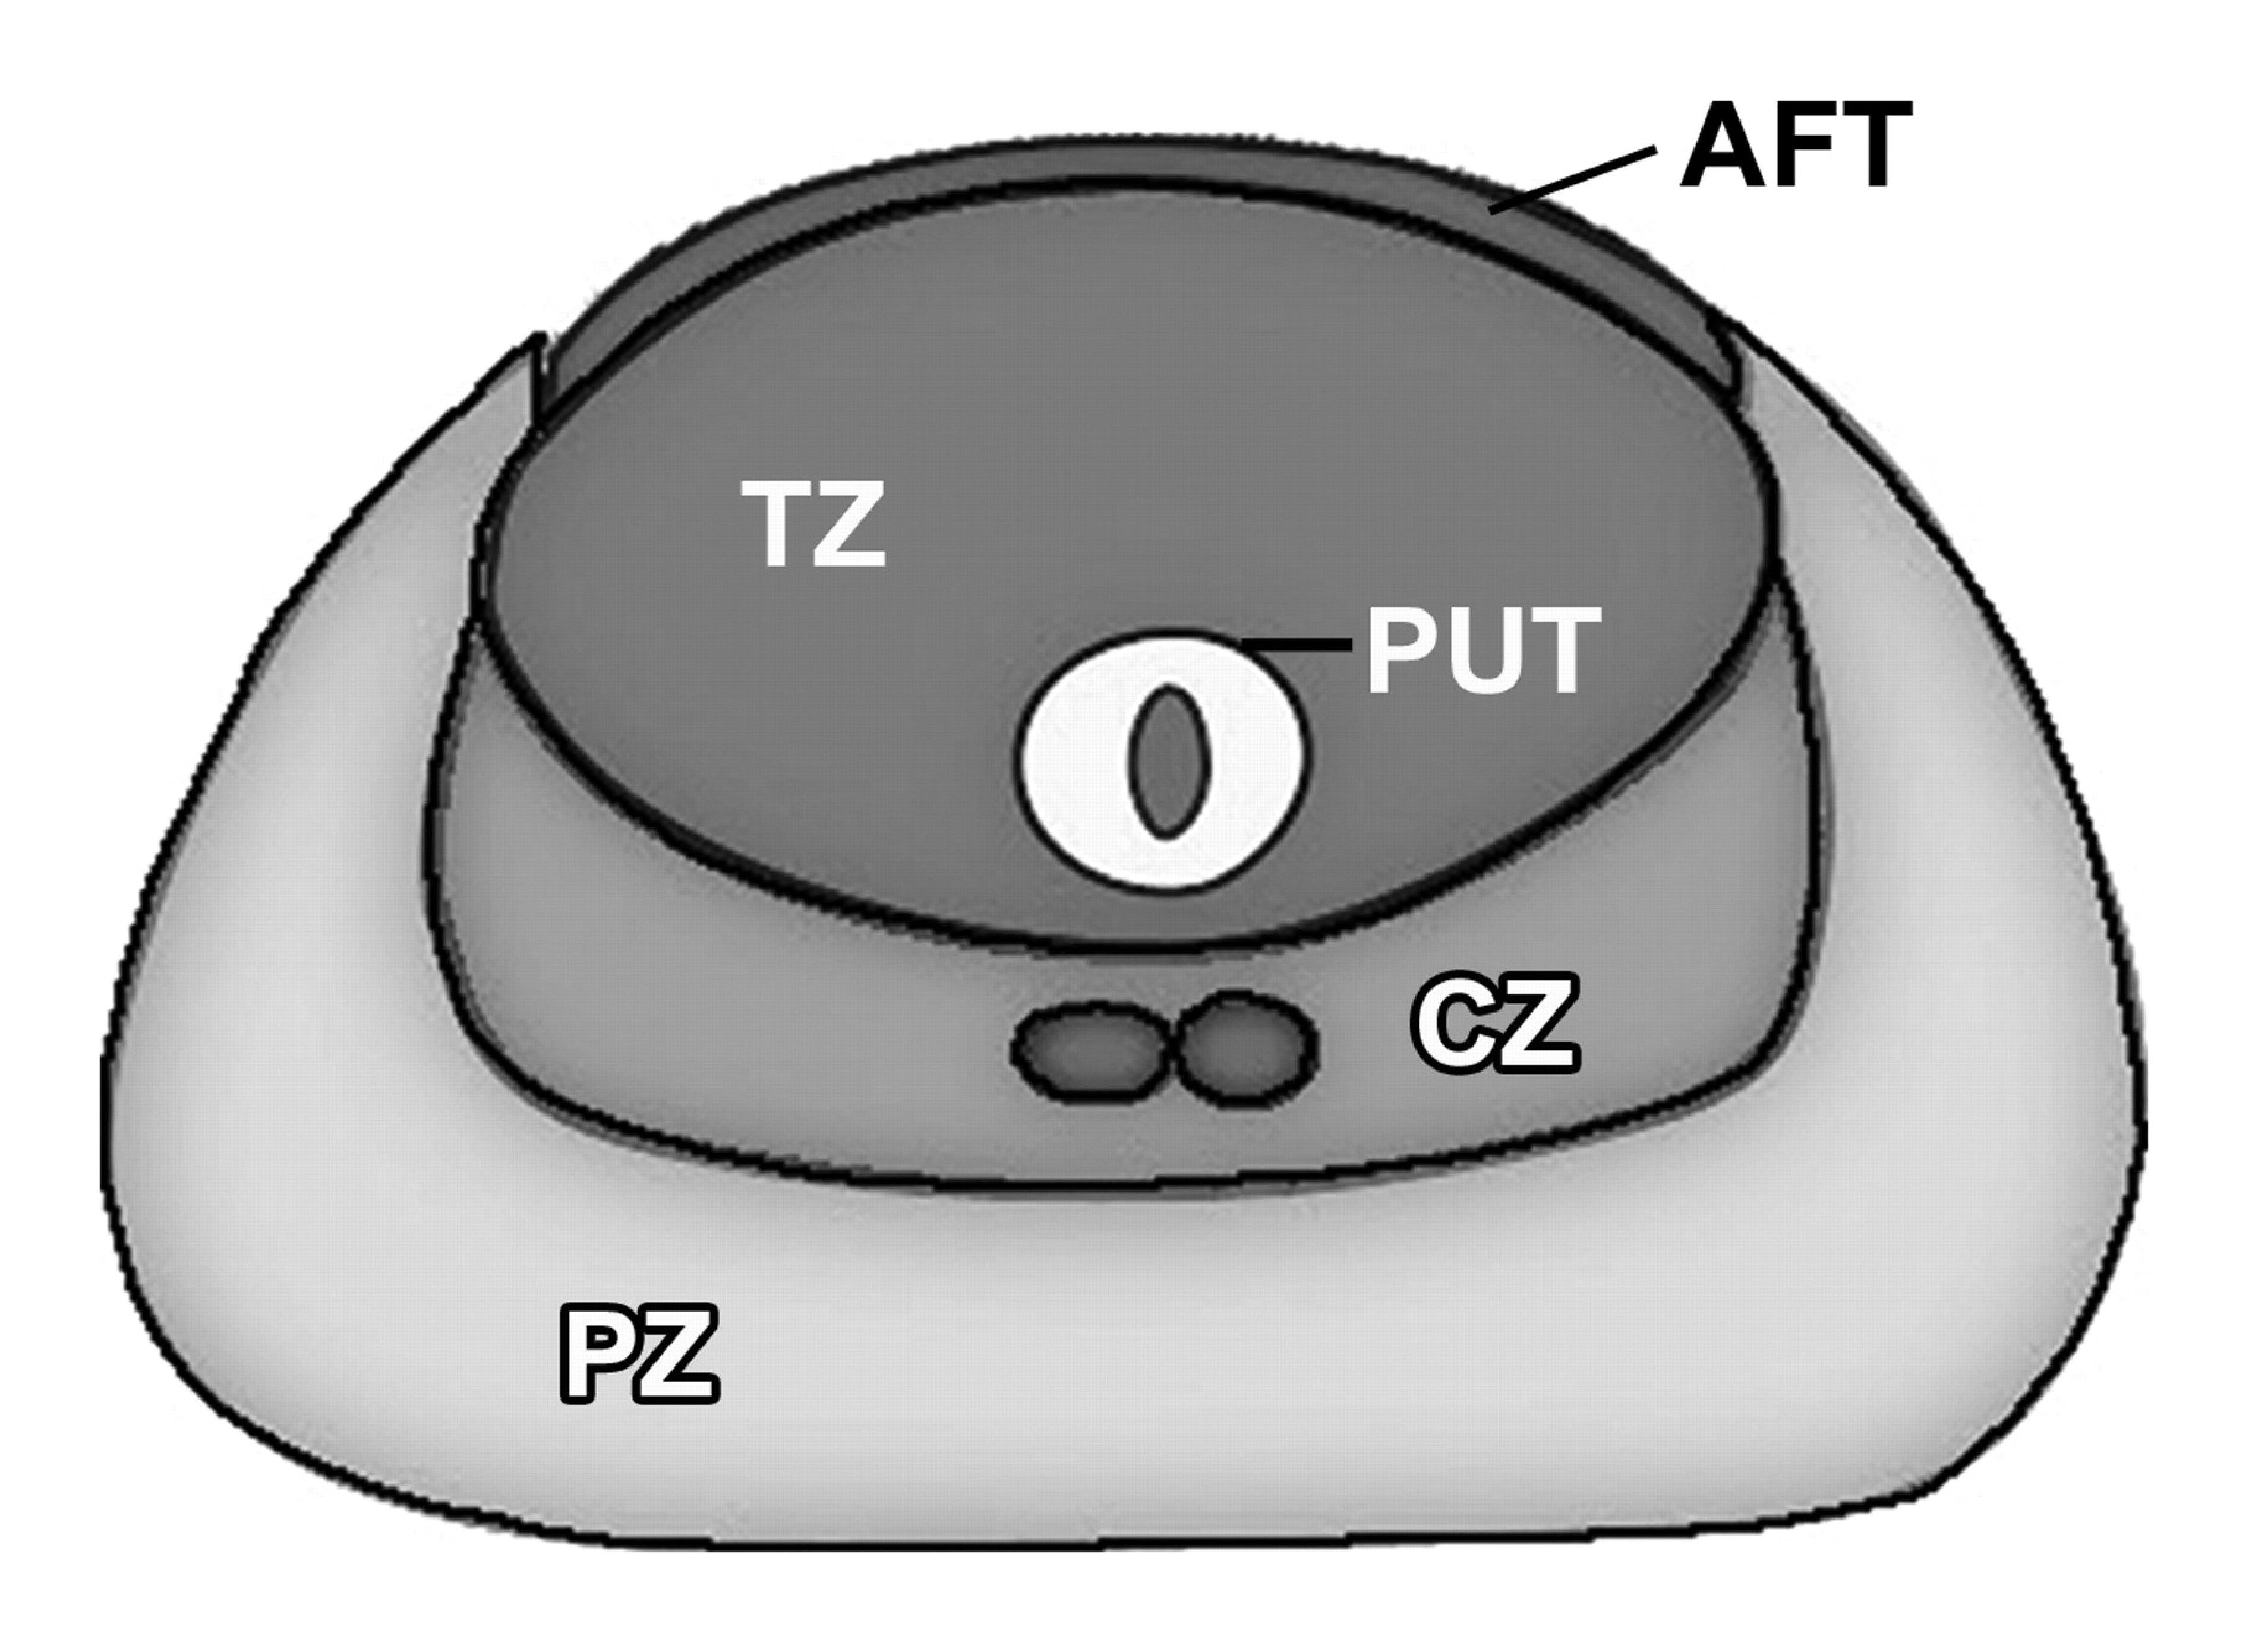
\includegraphics[height=0.15\textheight]{02_background/figures/anatomy/prostateTransverse.eps}
%			\label{fig:anatomyProstateTransverse}}
%			\hfill
%	\subfigure[Sagittal anatomy of the prostate.]{
%			\centering
%			\includegraphics[height=0.23\textheight]{02_background/figures/anatomy/prostateSagital.eps}
%			\label{fig:anatomyProstateSagittal}}\hspace*{\fill}
%	\caption{Prostate anatomy with division in different zones. \textit{AFT:} anterior fibromuscular tissue, \textit{CZ:} central zone, \textit{ED:} ejaculatory duct, \textit{NVB:} neurovascular bundle, \textit{PUT:}  tissue, \textit{PZ:} peripheral zone, \textit{U:} urethra, \textit{TZ:} transitional zone, \textit{B:} base, \textit{M:} median, \textit{A:} apex (copyright by \cite{Choi2007}).}
%	\label{fig:anatomyProstateZone}
%\end{figure*}
%
%The prostate is an exocrine gland of the male reproductive system having an inverted pyramidal shape. It measures approximately three centimetres in height by two and half centimetres in depth and its weight is estimated to be between seven and sixteen grams for an adult (\cite{Leissner1979}). The prostate size increases at two distinct stages during physical development: initially at puberty to reach its normal size, then again after sixty years of age leading to \ac{bph} (\cite{Parfait2010}).
%
%A zonal classification of the prostate, depicted in \acs{fig} \ref{fig:anatomyProstateZone}, was suggested by McNeal (\cite{McNeal1981}). Subsequently, this categorization was widely accepted in the literature (cf., \cite{Hricak1987,Villers1991,Coakley2000,Parfait2010}) and is used in all medical examinations (e.g., biopsy, \ac{mri} screening). The classification is based on dividing the gland into three distinct regions: (i) \ac{cz} accounting for 20-25\% of the whole prostate gland, (ii) \ac{tz} standing for 5\% and (iii) \ac{pz} representing the 70\%. In \ac{mri} images, tissues of \ac{cz} and \ac{tz} are difficult to distinguish and are usually merged into a common region, denominated \ac{cg}. As part of this classification, the prostate can be divided in three longitudinal portions depicted in \acs{fig} \ref{fig:anatomyProstateSagittal}: (i) base, (ii) median gland and (iii) apex.

\subsection{Prostate carcinoma}\label{subsec:procar}

\ac{cap} has been reported on a worldwide scale to be the second most frequently diagnosed cancer of men accounting for $13.6 \%$ (\cite{Ferlay2010}). Statistically, in 2008, the number of new diagnosed cases was estimated to be $899,000$ with no less than $258,100$ deaths (\cite{Ferlay2010}). In United States, aside from skin cancer, \ac{cap} was declared to be the most commonly diagnosed cancer among men, implying that approximately one in six men will be diagnosed with \ac{cap} during their lifetime and one in thirty-six will die from this disease causing \ac{cap} to be the second most common cause of cancer death among men (\cite{Siegel2013}, \cite{Society2013}).

Despite active research to determine the causes of prostate cancer, a fuzzy list of risk factors has been established (\cite{Society2010}). The etiology was linked to the following factors (\cite{Society2010}): (i) family history (\cite{Giovannucci2007,Steinberg1990}), (ii) genetic factors (\cite{Freedman2006,Amundadottir2006,Agalliu2009}), (iii) race-ethnicity (\cite{Giovannucci2007,Hoffman2001}), (iv) diet (\cite{Giovannucci2007,Ma2009,Alexander2010}), (v) obesity (\cite{Giovannucci2007,Rodriguez2007}). This list of risk factors alone cannot be used to diagnose CaP and in this way, screening enables early detection and treatment.

\ac{cap} growth is characterized by two main types of evolution (\cite{Strum2005}): slow and fast. The slow-growing tumours, accounting for up to 85 \% of all \acp{cap} (\cite{Lu-Yao2009}), progress slowly and usually stay confined to the prostate gland. For such cases, treatment can be substituted with active surveillance. In contrast, the second variant of \acp{cap} develops rapidly and metastasises from prostate gland to other organs, primarily the bones (\cite{Oster2013}). Bone metastases, being an incurable disease, significantly affect the morbidity and mortality rate (\cite{Ye2007}). Hence, the  results of the surveillance have to be trustworthy in order to distinguish aggressive from slow-growing \ac{cap}.

\ac{cap} is more likely to develop in specific regions of the prostate. In that respect, around 70-80 \% of \acp{cap} originate in \ac{pz} whereas 10-20 \% in \ac{tz} (\cite{Carrol1987,McNeal1988,Stamey1998}). Only about 5 \% of \acp{cap} occur in \ac{cz} (\cite{McNeal1988,Cohen2008}). However, those cancers appear to be more aggressive and more likely to invade other organs due to their location (\cite{Cohen2008}).

\subsection{\ac{cap} screening and imaging techniques}

\subsubsection{Current \ac{cap} screening}\label{subsubsec:curscr}

Current \ac{cap} screening consists of three different stages. First, \ac{psa} control is performed to distinguish between low and high risk \ac{cap}. Then, for confirmation, samples are taken during prostate biopsy and finally analysed to evaluate the prognosis and the stage of \ac{cap}. In this section, we present a detailed description of the current screening as well as its drawbacks.

Since its introduction in mid-1980s, \ac{psa} is widely used for \ac{cap} screening (\cite{Etzioni2002}). A higher-than-normal level of \ac{psa} can indicate an abnormality of the prostate either as a \ac{bph} or a cancer (\cite{Hoeks2011}). However, other factors can lead to an increased \ac{psa} level such as prostate infections, irritations, a recent ejaculation or a recent rectal examination (\cite{Parfait2010}).% \ac{psa} can be found in the bloodstream in two different forms: free \ac{psa} (about 10\%), and linked to another protein (about 90\%). A level of \ac{psa} higher than 10 ng.mL$^{-1}$ is considered to be at risk (\cite{Parfait2010}). If the \ac{psa} level is between 10 ng.mL$^{-1}$ and 4 ng.mL$^{-1}$, the patient is considered as suspicious (\cite{Barentsz2012}). In that case, the ratio of free \ac{psa} to total \ac{psa} is computed; if the ratio is higher than 15\%, the case is considered as pathological (\cite{Parfait2010}).

\Iac{trus} biopsy is carried out for cases which are considered as pathological. At least six different samples are taken randomly from the right and left parts of three three different zones: apex, median and base. These samples are further evaluated using the Gleason grading system (\cite{Gleason1977}). %The scoring scheme to characterize the biopsy sample is composed of five different patterns which correspond to grades ranging from 1 to 5. Higher grades are associated with poor prognosis (\cite{Epstein2005}). Then, in the Gleason system, two scores are assigned corresponding to (i) the grade of the most present tumour pattern, and (ii) the grade of the second most present tumour pattern (\cite{Epstein2005}). A higher \ac{gs} indicates a more aggressive tumour (\cite{Epstein2005}).
Also, it should be noted that biopsy is an invasive procedure which can result in serious infection or urine retention (\cite{Hara2005,Chou2011}).

Although \ac{psa} screening has been shown to improve early detection of \ac{cap} (\cite{Chou2011}), its lack of reliability motivates further investigations using \ac{mri}. Two reliable studies, carried out in the United States (\cite{Andriole2009}) and in Europe (\cite{Schroeder2012, Hugosson2010}), have attempted to assess the impact of early detection of \ac{cap}, with diverging outcomes (\cite{Chou2011,Heidenreich2013}). The study carried out in Europe\footnote{The \ac{ersspc}  started in the 1990s in order to evaluate the effect of \ac{psa} screening on mortality rate.} concluded that \ac{psa} screening reduces CaP-related mortality by 21-44\% (\cite{Schroeder2012, Hugosson2010}), while the American\footnote{The \ac{plco} cancer screening trial is carried out in the United States and intends to ascertain the effects of screening on mortality rate.} trial found no such effect (\cite{Andriole2009}). However, both studies agree that \ac{psa} screening suffers from low specificity, with an estimated rate of 36 \% (\cite{Schroder2008}). Both studies also agree that over-treatment is an issue: decision making regarding treatment is further complicated by difficulties in evaluating the aggressiveness and progression of \ac{cap} (\cite{Delpierre2013}). 

Hence, new screening methods should be developed with improved specificity of detection as well as more accurate risk assessment (aggressiveness and progression). Current research is focused on identifying new biological markers to replace \ac{psa}-based screening (\cite{Bourdoumis2010,Morgan2011,Brenner2013}). Until such research comes to fruition, these needs can be met through active-surveillance strategy using multi-parametric \ac{mri} techniques (\cite{Hoeks2011,Moore2013}). An \ac{mri}-\acs{cad} system, which is an area of active research and forms the focus of this paper, can be incorporated into this screening strategy allowing a more systematic and rigorous follow-up.

Another weakness of the current screening strategy lies in the fact that \ac{trus} biopsy does not provide trustworthy results. Due to its ``blind'' nature imposed by the a random sampling strategy, there is a chance of missing aggressive tumours or detecting microfocal ``cancers'', which influences the aggressiveness-assessment procedure (\cite{Noguchi2001}). As a consequence, over-diagnosis is estimated at up to 30 \% (\cite{Haas2007}), while missing clinically significant \ac{cap} is estimated at up to 35 \% (\cite{Taira2010}). In an effort to solve both issues, alternative biopsy approaches have been explored. \ac{mri}/\ac{us}-guided biopsy has been shown to outperform standard \ac{trus} biopsy (\cite{Delongchamps2013}). There, multimodal \ac{mri} images are fused with \ac{us} images in order to improve localization and aggressiveness assessment to carry out biopsies. Human interaction plays a major role in biopsy sampling which can lead to low repeatability; by reducing potential human errors at this stage, the \acs{cad} framework can be used to improve repeatability of examination.

\ac{cap} detection and diagnosis benefit from the use of \acs{cad} and \ac{mri} techniques. In the following sections, these techniques will be presented in addition to an overview of \acs{cad} for \ac{cap}.

\subsubsection{\ac{mri} imaging techniques}\label{subsubsec:mrimrsi}

\ac{mri} provides promising imaging techniques to overcome the previous mentioned drawbacks. Unlike \ac{trus} biopsy, \ac{mri} examination is a non-invasive protocol and has been shown to be the most accurate and harmless technique currently available (\cite{Turkbey2012}). In this section, we review different \ac{mri} modalities deveoped for \ac{cap} detection and diagnosis. Features used by the radiologist in their daily diagnosis task will receive particular attention together with their drawbacks. Moreover, these features commonly form the basis for developing analytic tools and automatic algorithms. However, we refer the reader to \acs{sec} \ref{subsec:featuredetection} for more details on automatic feature detection methods since they are part and parcel of the \acs{cad} framework. Table \ref{tab:modmri} provides an overview of the following discussion.

\begin{table*}
\begin{adjustwidth}{-1.5cm}{}
\caption{Overview of the features associated with each \ac{mri} modality used for medical diagnosis by radiologists. Acronyms: \acf{cap} - \acf{si} - \acf{gs}.}	
\begin{threeparttable}
\centering
\small
\renewcommand{\arraystretch}{1.2}
	\begin{tabular}{|m{1.7cm}||m{4.5cm}|>{\centering\arraybackslash}m{3.5cm}|>{\centering\arraybackslash}m{4cm}|>{\centering\arraybackslash}m{2cm}|}\hline
	\rowcolor{gray!10}
	Modality & Significant features & \ac{cap} & Healthy tissue & \ac{gs} correlation \\ \hline \hline
	\ac{t2w} \ac{mri} & \acs{si} & low-\ac{si} & intermediate to high-\ac{si} & + \\ \hline
	T$_2$ map & \acs{si} & low-\ac{si} & intermediate to high-\ac{si} & + \\ \hline
	\multirow{9}{*}{\ac{dce} \ac{mri}} & Semi-quantitative features: & & & \\[-1.5ex]
	& $-$ wash-in & faster & slower & 0 \\[-1.5ex]
	& $-$ wash-out & faster & slower & 0 \\[-1.5ex]
	& $-$ integral under the curve & higher & lower & 0 \\[-1.5ex]
	& $-$ maximum signal intensity & higher & lower & 0 \\[-1.5ex]
	& $-$ time-to-peak enhancement & faster & slower & 0 \\ \cline{2-5}
	& Quantitative features (Tofts' parameters): & & & \\[-1.5ex]
	& $-$ $\text{k}_{\text{ep}}$ & higher & lower & 0 \\[-1.5ex]
	& $-$ $\text{K}^{\text{trans}}$ & higher & lower & 0 \\ \hline
	\ac{dw} \ac{mri} & \acs{si} & higher-\ac{si} & lower-\ac{si} & + \\ \hline
	\acs{adc} map & \acs{si} & low-\ac{si} & high-\ac{si} & + \\ \hline
	\multirow{4}{*}{\ac{mrsi}}& Metabolites: & & & \\[-1.5ex]
	& Citrate (2.64 ppm) & lower concentration & higher concentration & + \\[-1.5ex]
	& Choline (3.21 ppm) & higher concentration & lower concentration & 0 \\[-1.5ex]
	& Spermine (3.11 ppm) & lower concentration & higher concentration & + \\ \hline
	
	\end{tabular}
	\begin{tablenotes}
      \small
      \item Notes:
      \item + = significantly correlated.
      \item 0 = no correlation.
    \end{tablenotes}
\end{threeparttable}
\end{adjustwidth}
\label{tab:modmri}
\end{table*}

\begin{figure*}
\centering

% Define block styles used later

\tikzstyle{module}=[draw, draw=blue!80, text width=10em, 
    text centered, minimum height=5em, minimum width = 15em, drop shadow, rounded corners,
    fill=blue!30]
    
\tikzstyle{vecArrow} = [thick, decoration={markings,mark=at position
   1 with {\arrow[semithick]{open triangle 60}}},
   double distance=1.4pt, shorten >= 5.5pt,
   preaction = {decorate},
   postaction = {draw,line width=1.4pt, white,shorten >= 4.5pt}]

% Define distances for bordering
\def\blockdist{1.5}
\def\edgedist{2.5}

\begin{tikzpicture}[node distance=3cm,thick,scale=0.6, every node/.style={scale=0.6},path image/.style={
path picture={
\node at (path picture bounding box.center) {
\includegraphics[width=1cm]{#1}
};}}]
\tikzstyle{conefill} = [path image=,fill opacity=0.8]
\node[module=above:pre] (pre) at (4.5,-2.6) {\Large Pre-processing};
\node[module,below of=pre] (seg) {\Large Segmentation};
\node[module,below of=seg] (reg) {\Large Registration};

\path[->,dashed] (seg.west) edge [bend right=70] node {} (reg.west);
\path[->,dashed] (reg.east) edge [bend right=70] node {} (seg.east);

\draw[->] (pre)--(seg);
\draw[->] (seg)--(reg);

\begin{pgfonlayer}{background}
	\path (pre.west |- pre.north)+(-0.9,1.0+\blockdist) node (a) {};
    \path (reg.east |- reg.south)+(+0.9,-0.5) node (b) {};
          
    \path[fill=blue!10,rounded corners, draw=blue!20, dashed] (a) rectangle (b);
\end{pgfonlayer}
        
\path (pre.north) +(0,+\blockdist) node (bgreg) {\Large Image regularization};

\begin{scope}[node distance=10cm]
	\node[module] (det) [below right=0cm and 3cm of pre] {\Large Features detection};
\end{scope}
\begin{scope}[node distance=3.5cm]
	\node[module,above of=det] (roi) {\Large ROIs\\detection/selection};
\end{scope}
\node[module,below of=det] (sel) {\Large Features\\selection/extraction};
\node[module,below of=sel] (cla) {\Large Features\\classification/fusion};

\draw[->] (roi)--(det);
\draw[->] (det)--(sel);
\draw[->] (sel)--(cla);

%\begin{pgfonlayer}{background}
%	\path (roi.west |- roi.north)+(-0.5,1.0+\blockdist) node (c) {};
%    \path (cla.east |- cla.south)+(+0.5,-0.5) node (d) {};
%          
%    \path[fill=blue!10,rounded corners, draw=blue!20, dashed] (c) rectangle (d);
%\end{pgfonlayer}
%
%\path (roi.north) +(0,+\blockdist) node (bgfea) {\Large Image classification};

\begin{pgfonlayer}{background}
	\path (roi.west |- roi.north)+(-0.25,0.8) node (c) {};
    \path (roi.east |- roi.south)+(+0.25,-0.25) node (d) {};
          
    \path[fill=blue!20,rounded corners, draw=blue!25, dashed] (c) rectangle (d);
\end{pgfonlayer}

\path (roi.west |- roi.north) +(.6,0.4) node (bgfea) {\Large \textbf{CADe}};

\begin{pgfonlayer}{background}
	\path (det.west |- det.north)+(-0.25,0.8) node (c) {};
    \path (cla.east |- cla.south)+(+0.25,-0.25) node (d) {};
          
    \path[fill=blue!20,rounded corners, draw=blue!25, dashed] (c) rectangle (d);
\end{pgfonlayer}

\path (roi.west |- det.north) +(.6,0.4) node (bgfea) {\Large \textbf{CADx}};     

% Define the place where the arrow should start anf finish
\path (seg.east |- seg.north)+(+0.9,0) node (e) {};
\path (sel.west |- seg.north)+(-0.8,0) node (f) {};

\draw[double distance =3pt,preaction={-triangle 90,thin,draw,shorten >=-1mm}] (e) -- (f) node[midway,above] {\Large Regularized data};

\begin{scope}[yshift=34,xshift=-86]
	\transparent{0.6}\draw[path image=02_background/figures/tikzimage/t2.eps] (0,0) rectangle (1.0,1.0);
\end{scope}

\begin{scope}[yshift=31,xshift=-83]
	\transparent{0.6}\draw[path image=02_background/figures/tikzimage/t2.eps] (0,0) rectangle (1.0,1.0);
\end{scope}

\begin{scope}[yshift=28,xshift=-80]
	\transparent{0.8}\draw[path image=02_background/figures/tikzimage/t2.eps] (0,0) rectangle (1.0,1.0);
	\path (0,0)+(-1.5,0.3) node {\Large T$_2$-W MRI};
\end{scope}

\begin{scope}[yshift=-33,xshift=-86]
	\transparent{0.6}\draw[path image=02_background/figures/tikzimage/t2.eps] (0,0) rectangle (1.0,1.0);
\end{scope}

\begin{scope}[yshift=-36,xshift=-83]
	\transparent{0.6}\draw[path image=02_background/figures/tikzimage/t2.eps] (0,0) rectangle (1.0,1.0);
\end{scope}

\begin{scope}[yshift=-39,xshift=-80]
	\transparent{0.8}\draw[path image=02_background/figures/tikzimage/t2.eps] (0,0) rectangle (1.0,1.0);
	\path (0,0)+(-1.2,0.3) node {\Large T$_2$ map};
\end{scope}

\begin{scope}[yshift=-100,xshift=-86]
	\transparent{0.6}\draw[path image=02_background/figures/tikzimage/dce.eps] (0,0) rectangle (1.0,1.0);
\end{scope}

\begin{scope}[yshift=-103,xshift=-83]
	\transparent{0.6}\draw[path image=02_background/figures/tikzimage/dce.eps] (0,0) rectangle (1.0,1.0);
\end{scope}

\begin{scope}[yshift=-106,xshift=-80]
	\transparent{0.8}\draw[path image=02_background/figures/tikzimage/dce.eps] (0,0) rectangle (1.0,1.0);
	\path (0,0)+(-1.5,0.3) node {\Large DCE MRI};
\end{scope}

\begin{scope}[yshift=-167,xshift=-86]
	\transparent{0.6}\draw[path image=02_background/figures/tikzimage/dwi1.eps] (0,0) rectangle (1.0,1.0);
\end{scope}

\begin{scope}[yshift=-170,xshift=-83]
	\transparent{0.6}\draw[path image=02_background/figures/tikzimage/dwi1.eps] (0,0) rectangle (1.0,1.0);
\end{scope}

\begin{scope}[yshift=-173,xshift=-80]
	\transparent{0.8}\draw[path image=02_background/figures/tikzimage/dwi1.eps] (0,0) rectangle (1.0,1.0);
	\path (0,0)+(-1.5,0.3) node {\Large DW MRI};
\end{scope}

\begin{scope}[yshift=-234,xshift=-86]
\transparent{0.6}\draw[path image=02_background/figures/tikzimage/adc.eps] (0,0) rectangle (1.0,1.0);
\end{scope}

\begin{scope}[yshift=-237,xshift=-83]
\transparent{0.6}\draw[path image=02_background/figures/tikzimage/adc.eps] (0,0) rectangle (1.0,1.0);
\end{scope}

\begin{scope}[yshift=-240,xshift=-80]
\transparent{0.8}\draw[path image=02_background/figures/tikzimage/adc.eps] (0,0) rectangle (1.0,1.0);
	\path (0,0)+(-1.5,0.3) node {\Large ADC};
\end{scope}

\begin{scope}[yshift=-301,xshift=-86]
	\transparent{0.6}\draw[path image=02_background/figures/tikzimage/mrsi.eps] (0,0) rectangle (1.0,1.0);
\end{scope}

\begin{scope}[yshift=-304,xshift=-83]
\transparent{0.6}\draw[path image=02_background/figures/tikzimage/mrsi.eps] (0,0) rectangle (1.0,1.0);
\end{scope}

\begin{scope}[yshift=-307,xshift=-80]
\transparent{0.8}\draw[path image=02_background/figures/tikzimage/mrsi.eps] (0,0) rectangle (1.0,1.0);
	\path (0,0)+(-1,0.3) node {\Large MRSI};
\end{scope}

\path (pre.west |- roi.north)+(-3.5,1.0+\blockdist) node (g) {};
\path (reg.west |- cla.south)+(-3.5,-0.5) node (h) {};

\draw[decorate,decoration={brace,raise=6pt,amplitude=10pt}, thick]
    (g)--(h) ;
    
\path (seg.west |- seg.north)+(-2.5,0) node (i) {};
\path (seg.west |- seg.north)+(-0.9,0) node (j) {};
   
\draw[double distance =3pt,preaction={-triangle 90,thin,draw,shorten >=-1mm}] (i) -- (j);   

\path (sel.east |- seg.north)+(2,0) node (k) {};
\path (sel.east |- seg.north)+(0.5,0) node (l) {};
   
%\draw[double distance =3pt,preaction={-triangle 90,thin,draw,shorten >=-1mm}] (l) -- (k);  
%
%\begin{scope}[path image/.style={
%path picture={
%\node at (path picture bounding box.center) {
%\includegraphics[width=3cm]{#1}
%};}}]    
%\begin{scope}[yshift=-180,xshift=560]
%	\transparent{0.6}\draw[path image=02_background/figures/tikzimage/likeli.eps,very thin] (0,0) rectangle (3.0,3.0);
%\end{scope}
%
%\begin{scope}[yshift=-175,xshift=570]
%\transparent{0.6}\draw[path image=02_background/figures/tikzimage/likeli.eps,very thin] (0,0) rectangle (3.0,3.0);
%\end{scope}
%
%\begin{scope}[yshift=-170,xshift=580]
%	\transparent{0.8}\draw[path image=02_background/figures/tikzimage/likeli.eps,very thin] (0,0) rectangle (3.0,3.0);
%	\path (0,0)+(+1,-1) node {\Large Likelihood};
%	\path (0,0)+(+1,-1.5) node {\Large cancer};
%	\path (0,0)+(+1,-2) node {\Large map};
%\end{scope}
%\end{scope}
\end{tikzpicture}
\caption{Common \ac{cad} framework based on \ac{mri} images used to detect \ac{cap}.}
\label{fig:wkfcad}
\end{figure*}

% We are using enumerate with a small margin and some indent to organize our thoughts by paragraphs.
\setenumerate{listparindent=\parindent,itemsep=10px}
\setlist{noitemsep}
\begin{enumerate}[leftmargin=*]

\begin{figure*}
\centering
	\hspace*{\fill}
	\subfigure[\ac{t2w}-\ac{mri} slice of an healthy prostate acquire with a 1.5 Tesla \ac{mri}. The blue contour represents the \ac{cg} while the \ac{pz} corresponds to the green contour.]{\label{subfig:t2whealthy}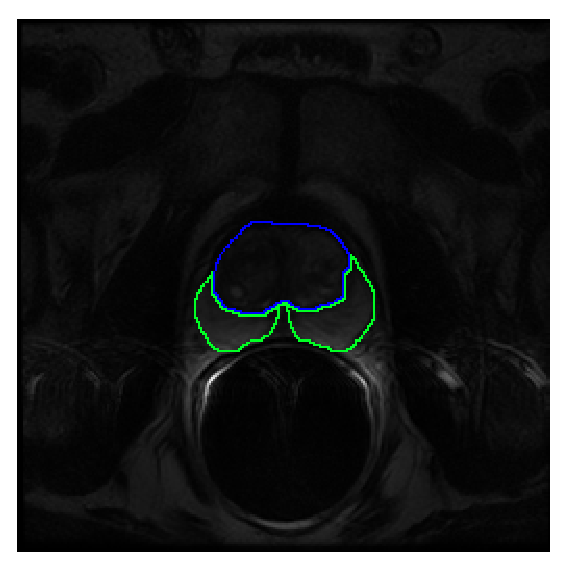
\includegraphics[width=0.3\linewidth]{02_background/figures/t2w/t2w_healthy.eps}} \hfill
	\subfigure[\ac{t2w}-\ac{mri} slice of a prostate with a \ac{cap} highlighted in the \ac{pz} using a 3.0 Tesla \ac{mri} scanner.]{\label{subfig:t2wcancerpz}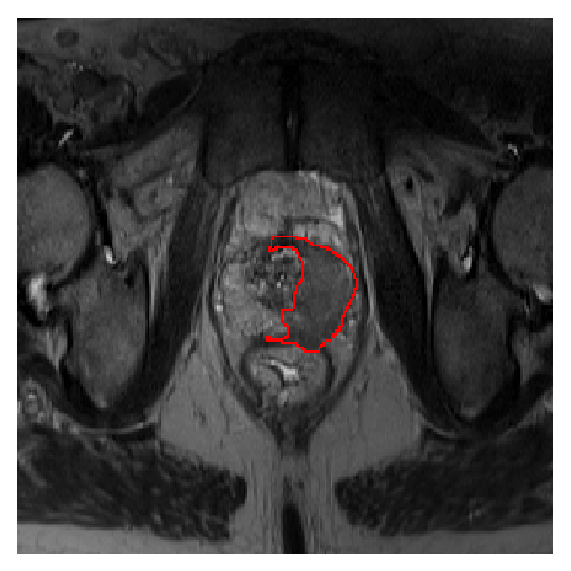
\includegraphics[width=0.3\linewidth]{02_background/figures/t2w/t2w_cancer_pz.eps}} \hfill
	\subfigure[\ac{t2w}-\ac{mri} slice of a prostate with a \ac{cap} highlighted in the \ac{cg} using a 3.0 Tesla \ac{mri} scanner.]{\label{subfig:t2wcancercg}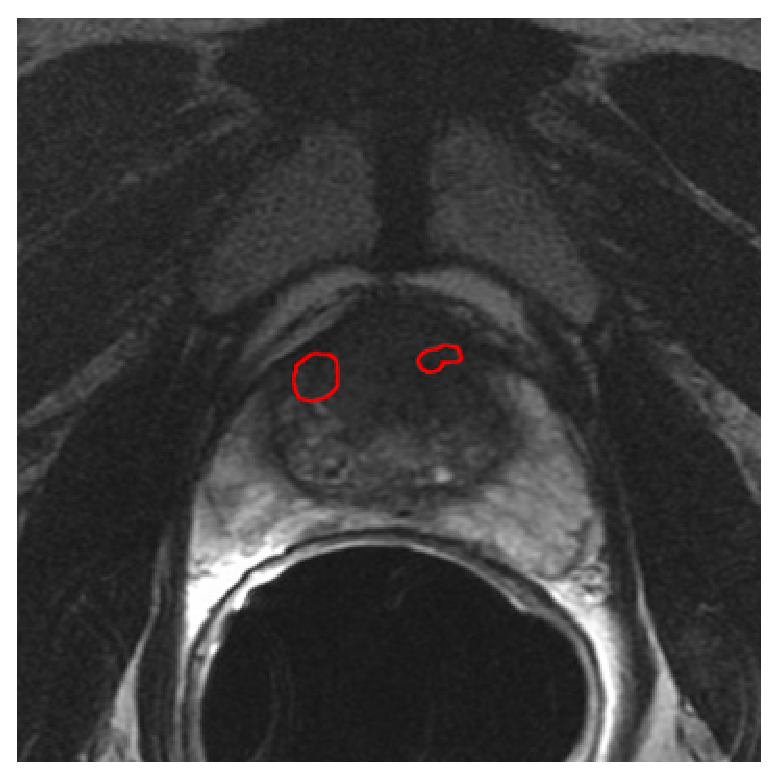
\includegraphics[width=0.3\linewidth]{02_background/figures/t2w/t2w_cancer_cg.eps}}
	\hspace*{\fill}
	\caption{Rendering of \ac{t2w}-\ac{mri} prostate image with both 1.5 and 3.0 Tesla \ac{mri} scanner.}
	\label{fig:t2w}
\end{figure*}

%T2W MRI
\item[$-$] \textbf{\textit{\ac{t2w} \ac{mri}:}} \ac{t2w} \ac{mri} was the first \ac{mri}-modality used to perform \ac{cap} diagnosis using \ac{mri} (\cite{Hricak1983}). Nowadays, radiologists make use of it for \ac{cap} detection, localization and staging purposes. This imaging technique is well suited to render zonal anatomy of the prostate (\cite{Barentsz2012}). 

%This modality relies on a sequence based on setting a long \ac{tr}, reducing the T$_1$ effect in \ac{nmr} signal measured, and fixing the \ac{te} to sufficiently large values in order to enhance the T$_2$ effect of tissues. Thus, 
\ac{pz} and \ac{cg} tissues are well perceptible in these images. The former is characterized by an intermediate/high-\ac{si} while the latter is depicted by a low-\ac{si} (\cite{Hricak1987}). An example of a healthy prostate is shown in Fig.~\ref{subfig:t2whealthy}.

In \ac{pz}, round or ill-defined low-SI masses are synonymous with \acp{cap} (\cite{Hricak1983}) as shown in Fig.~\ref{subfig:t2wcancerpz}. Detecting \ac{cap} in \ac{cg} is more challenging. In fact both normal \ac{cg} tissue and malignant tissue, have a low-\ac{si} in \ac{t2w} \ac{mri} reinforcing difficulties to distinguish between them. However, \acp{cap} in \ac{cg} appear often as homogeneous mass possessing ill-defined edges with lenticular or ``water-drop'' shapes (\cite{Akin2006, Barentsz2012}) as depicted in Fig.~\ref{subfig:t2wcancercg}. 

\ac{cap} aggressiveness was shown to be inversely correlated with \ac{si}. Indeed, \acp{cap} assessed with a \ac{gs} of 4-5 implied lower \ac{si} than the one with a \ac{gs} of 2-3 (\cite{Wang2008}).

In spite of the availability of these useful and encouraging features, the \ac{t2w} modality lacks reliability (\cite{Kirkham2006,Hoeks2011}). Sensitivity is affected by the difficulties in detecting cancers in \ac{cg} (\cite{Kirkham2006}) while specificity rate is highly affected by outliers (\cite{Barentsz2012}). In fact, various conditions emulate patterns of \ac{cap} such as \ac{bph}, post-biopsy haemorrhage, atrophy, scars and post-treatment (\cite{Hricak1987,Quint1991,Scheidler1999,Cruz2002,Barentsz2012}). These issues can be partly addressed using more innovative and advanced modalities such as later presented.

%T2 Map
\item[$-$] \textbf{\textit{T$_2$ Map:}} As previously mentioned, \ac{t2w} \ac{mri} modality shows low sensitivity due to various effects (\cite{Hegde2013}). However, T$_2$ values alone have been shown to be more discriminative (\cite{Liu2011}) and highly correlated with citrate concentration, a biological marker in \ac{cap} (\cite{Liney1996,Liney1997}). 

%T$_2$ values are computed using the characteristics of transverse relaxation. Transverse relaxation is formalized as:
%
%\begin{equation}
%	M_{x,y}(t) = M_{x,y}(0) \exp \left( - \frac{t}{\text{T}_2} \right) \ ,
%	\label{eq:tramag}
%\end{equation}
%
%\noindent where $M_{x,y}(0)$ is the initial value of $M_{x,y}(t)$ and T$_2$ is the relaxation time.
%
%By rearranging \acs{eq} \ref{eq:tramag}, T$_2$ map is computed performing a linear fitting on the model in \acs{eq} \ref{eq:t2map} using several TE, $t=\{ \text{TE}_1,\text{TE}_2, \dotsc ,\text{TE}_m \}$.
%
%\begin{equation}
%	\ln \left[ \frac{M_{x,y}(t)}{M_{x,y}(0)} \right] = - \frac{t}{\text{T}_2} \ .
%	\label{eq:t2map}
%\end{equation}

The \Ac{fse} sequence has been shown to be particularly well suited in order to build a T$_2$ map and obtain accurate T$_2$ values (\cite{Liney1996a}).

Similar to \ac{t2w} \ac{mri}, T$_2$ values associated with \ac{cap} are significantly lower than those of healthy tissues (\cite{Liney1996,Gibbs2001}).

%DCE MRI
\item[$-$] \textbf{\textit{\ac{dce} \ac{mri}:}} \ac{dce} \ac{mri} is an imaging technique which exploits the vascularity characteristic of tissues. Contrast media, usually gadolinium-based, is injected intravenously into the patient. The media extravasates from vessels to the \ac{ees} and is then released back into the vasculature before being eliminated by the kidneys (\cite{Gribbestad2005}). Furthermore, the diffusion speed of the contrast agent may vary due to several parameters: (i) the permeability of the micro-vessels, (ii) their surface area and (iii) the blood flow (\cite{Padhani2002}).

%Healthy \ac{pz} is mainly made up of glandular tissue, around 70 \% (\cite{Choi2007}), which implies a reduced interstitial space restricting exchanges between vessels and \ac{ees} (\cite{Buckley2004,Niekerk2009}). Normal \ac{cg} has a more disorganised structure, composed of mainly fibrous tissue (\cite{Choi2007,Hoeks2011}), which facilitates the arrival of the contrast agent in \ac{ees} (\cite{Niekerk2013}). To understand the difference between contrast media kinetic in malignant tumours and the two previous behaviours mentioned, one has to focus on the process known as angiogenesis (\cite{Carmeliet2000}). In order to ensure growth, malignant tumours produce and release angiogenic promoter substances (\cite{Carmeliet2000}). These molecules stimulate the creation of new vessels towards the tumour (\cite{Carmeliet2000}). However, the new vessel networks in tumours differ from those present in healthy tissue (\cite{Gribbestad2005}). They are more porous due to the fact that their capillary walls have a large number of ``openings'' (\cite{Gribbestad2005,Choi2007}). In contrast to healthy cases, this increased vascular permeability results in increased contrast agent exchanges between vessels and \ac{ees} (\cite{Verma2012}).

%By making use of the previous aspects, 
\ac{dce} \ac{mri} is based on an acquisition of a set of \ac{t1w} \ac{mri} images over time. the Gadolinium-based contrast agent shortens T$_1$ relaxation time enhancing contrast in \ac{t1w} \ac{mri} images. The aim is to post-analyse the pharmacokinetic behaviour of the contrast media concentration in prostate tissues (\cite{Verma2012}). The image analysis is carried out in two dimensions: (i) in the spatial domain on a pixel-by-pixel basis and (ii) in the time domain corresponding to the consecutive images acquired with the \ac{mri}. Thus, for each spatial location, a signal linked to contrast media concentration is measured as shown in Fig.~\ref{fig:dceana} (\cite{Tofts2010}). 
%By taking the previous remarks regarding medical aspects and signal theory into account, 
\acp{cap} are characterized by a signal having an earlier and faster enhancement as well as an earlier wash-out (cf., the rate of the contrast agent flowing out of the tissue) (see Fig.~\ref{subfig:dce}) (\cite{Verma2012}). Three different approaches exist to analyse these signals with the aim of tagging them as corresponding to either normal or malignant tissues. Qualitative analysis is based on assessment of the signal shape (\cite{Hoeks2011}). Quantitative approaches consist of inferring pharmocokinetic parameter values (\cite{Tofts2010}). Those parameters are part of mathematical-pharmacokinetic models which are directly based on physiological exchanges between vessels and \ac{ees}. % Several pharmacokinetic models were proposed such as the Kety model (\cite{Kety1951}), the Tofts model (\cite{Tofts1997}) and mixed models (\cite{Larsson1996,StLawrence1998}).
The last family of methods mix both approaches and are grouped together under the heading of semi-quantitative methods. They rely on shape characterization using mathematical modelling to extract a set of parameters. % such as wash-in gradient, wash-out, integral under the curve, maximum signal intensity, time-to-peak enhancement and start of enhancement.
These parameters will be discussed in a later section (see Fig.~\ref{fig:dceparam}) (\cite{Hoeks2011,Verma2012}). It was shown that semi-quantitative and quantitative methods improve localization of \ac{cap} when compared with qualitative methods (\cite{Rosenkrantz2013}). Section \ref{subsubsec:fddce} provides a full description of quantitative and semi-quantitative approaches.

\ac{dce} \ac{mri} combined with \ac{t2w} \ac{mri} has shown to enhance sensitivity compared to \ac{t2w} \ac{mri} alone (\cite{Jager1997,Kim2005,Schlemmer2004,Zelhof2009}). Despite this fact, \ac{dce} \ac{mri} possesses some drawbacks. Due to its ``dynamic'' nature, patient motions during the image acquisition may lead to spatial misregistration of the image set (\cite{Verma2012}). Furthermore, it has been suggested that malignant tumours are difficult to distinguish from prostatitis located in \ac{pz} and \ac{bph} located in \ac{cg} (\cite{Hoeks2011,Verma2012}) as these two pairs of tissues tend to have similar appearances. Later studies have shown that \acp{cap} in \ac{cg} do not always manifest in homogeneous fashion. Indeed, tumours in this zone can present both hypo-vascularization and hyper-vascularization which illustrates the challenge of \ac{cap} detection in \ac{cg} (\cite{Niekerk2013}).

\begin{figure*}
\centering
	\hspace*{\fill}
	\subfigure[\ac{t1w}-\ac{mri} image where the cancer is delimited by the red contour. The green area was still not invaded by the \ac{cap}]{\label{subfig:t1w}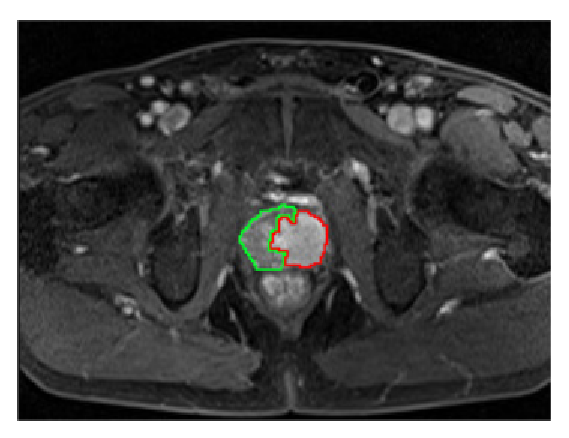
\includegraphics[width=0.4\linewidth]{02_background/figures/dce/slice.eps}} \hfill
	\subfigure[Enhancement curve computed during the \ac{dce}-\ac{mri} analysis. The red curve is typical from \ac{cap} cancer while the green curve is characteristic of healthy tissue.]{\label{subfig:dce}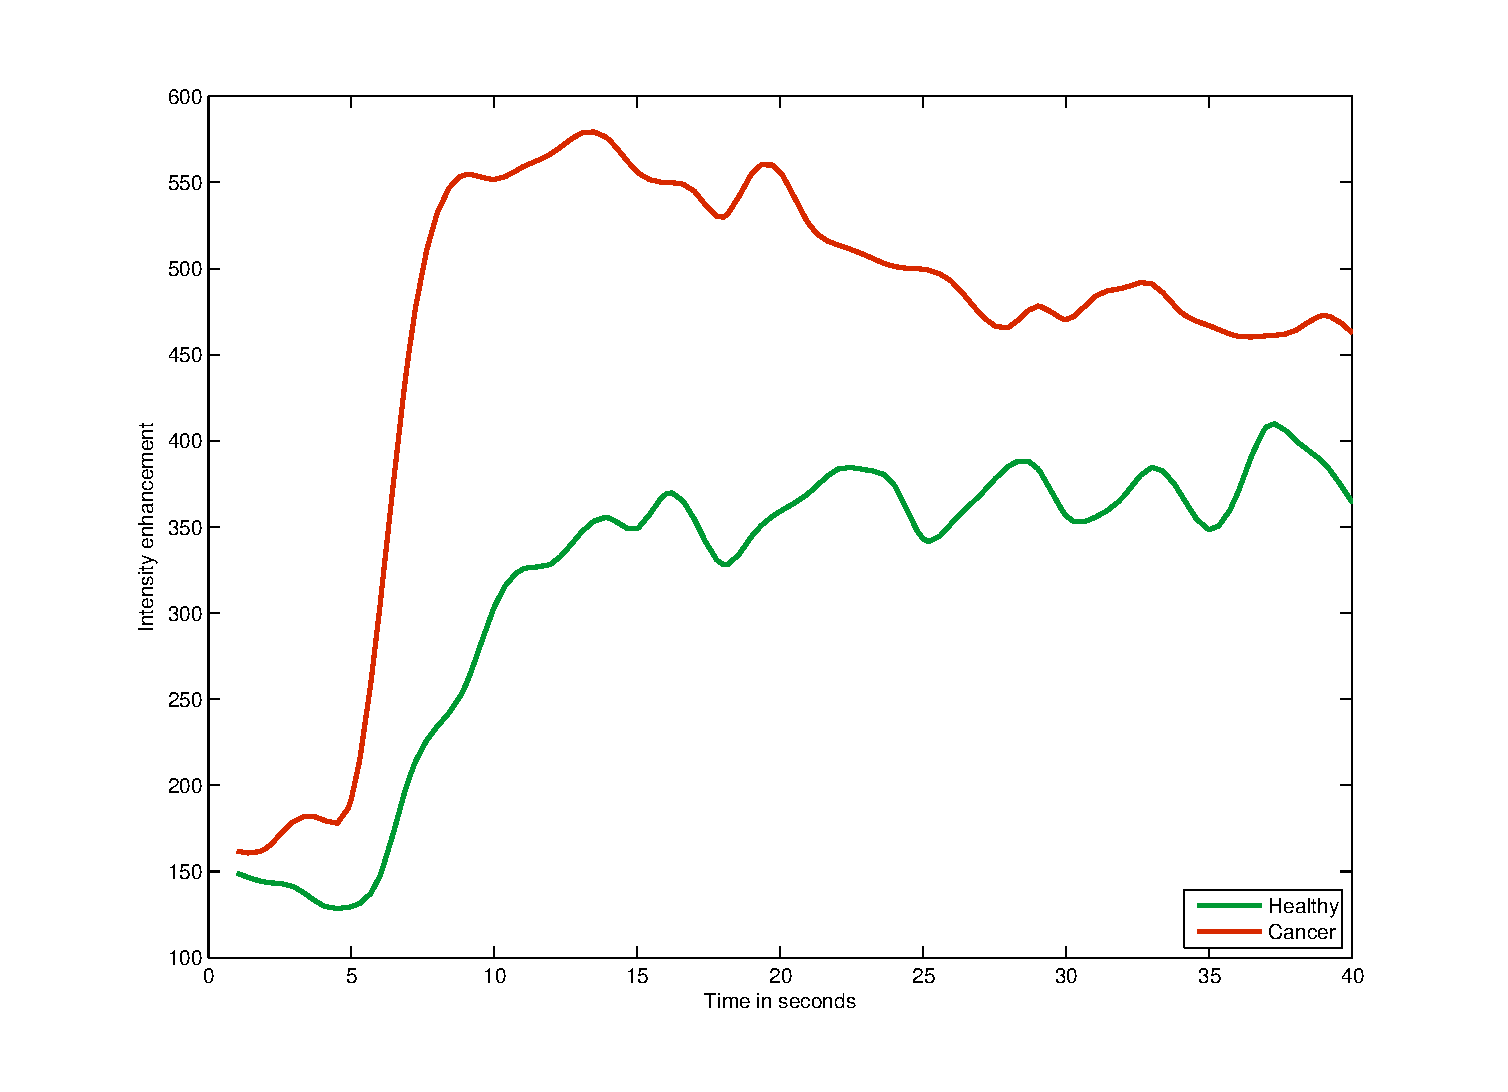
\includegraphics[width=0.45\linewidth]{02_background/figures/dce/dce_cancer_healthy.eps}}
	\hspace*{\fill}
	\caption{Illustration of typical enhancement signal observed in \ac{dce}-\ac{mri} analysis collected with a 3.0 Tesla \ac{mri} scanner.}
	\label{fig:dceana}
\end{figure*}

%DWI MRI
\item[$-$] \textbf{\textit{\ac{dw} \ac{mri}:}} As previously mentioned in the introduction, \ac{dw} \ac{mri} is the most recent MRI imaging technique aiming at \ac{cap} detection and diagnosis (\cite{Scheidler1999}). This modality exploits the variations in the motion of water molecules in different tissues (\cite{LeBihan1988,Koh2007}).

%From a physiological point of view, the following facts can be claimed. On the one hand, \ac{pz}, as previously mentioned, is mainly glandular and tubular in structure allowing water molecules to move freely (\cite{Choi2007,Hoeks2011}). On the other hand, \ac{cg} is made up of muscular or fibrous tissue causing the motion of the water molecules to be more constrained and heterogeneous than in \ac{pz} (\cite{Hoeks2011}). Then, \ac{cap} growth leads to the destruction of normal glandular structure and is associated with an increase in cellular density (\cite{Hoeks2011,Koh2007,Somford2008}). Furthermore, these factors both have been shown to be inversely correlated with water diffusion (\cite{Koh2007,Somford2008}): higher cellular density implies a restricted water diffusion. Thus, water diffusion in \ac{cap} will be more restricted than both healthy \ac{pz} and \ac{cg} (\cite{Koh2007,Hoeks2011}).

From the \ac{nmr} principle side, \ac{dw} \ac{mri} sequence produces contrasted images due to variation of water molecules motion. The method is based on the fact that the signal in \ac{dw} \ac{mri} images is inversely correlated to the degree of random motion of water molecules (\cite{Huisman2003}). % In fact, gradients are used in \ac{dw} \ac{mri} modality to encode spatial location of nuclei temporarily. Simplifying the problem in only one direction, a gradient is applied in that direction, dephasing the spins of water nuclei. Hence, the spin phases vary along the gradient direction depending of the gradient intensity at those locations. Then, a second gradient is applied aiming at cancelling the spin dephasing. Thus, the immobile water molecules will be subject to the same gradient intensity as the initial one while moving water molecules will be subject to a different gradient intensity. Thus, spins of moving water molecules will stay dephased whereas spins of immobile water molecules will come back in phase. As a consequence, 
A higher degree of random motion results in a more significant signal loss whereas a lower degree of random motion is synonymous with lower signal loss (\cite{Huisman2003}). Under these conditions, the MRI signal is measured as:

\begin{equation}
	M_{x,y}\left(t,b\right) = M_{x,y}(0) \exp \left( - \frac{t}{\text{T}_2} \right) S_{\text{ADC}}(b) \ , 
	\label{eq:t2dif}
\end{equation}

\begin{equation}
	S_{\text{ADC}}(b) = \exp \left( -b \times \text{ADC} \right) \ ,
	\label{eq:dif}
\end{equation}

\noindent where $S_{\text{ADC}}$ refers to signal drop due to diffusion effect, $\text{ADC}$ is the \acl{adc} and $b$ is the attenuation coefficient depending only on gradient pulses parameters: (i) gradient intensity and (ii) gradient duration (\cite{LeBihan1986}).

By using this formulation, image acquisition with a parameter $b=0$ s.mm$^{-2}$ corresponds to a \ac{t2w} \ac{mri} acquisition. Then, increasing the attenuation coefficient $b$ (cf., increase gradient intensity and duration) enhances the contrast in \ac{dw} \ac{mri} images.

To summarize, in \ac{dw} \ac{mri} images, \acp{cap} are characterized by high-\ac{si} compared to normal tissues in \ac{pz} and \ac{cg} as shown in Fig.~\ref{subfig:dwi} (\cite{Barentsz2012}). However, some tissues in \ac{cg} can look similar to \ac{cap} with higher \ac{si} (\cite{Barentsz2012}).

Diagnosis using \ac{dw} \ac{mri} combined with \ac{t2w} \ac{mri} has shown a significant improvement compared with \ac{t2w} \ac{mri} alone and provides highly contrasted images (\cite{Shimofusa2005,Padhani2011,Choi2007}). As drawbacks, this modality suffers from poor spatial resolution and low specificity due to false positive detection (\cite{Choi2007}).

With a view to eliminate these drawbacks, radiologists are extracting quantitative maps from \ac{dw} \ac{mri}. This imaging technique is presented next.

\begin{figure}
\centering
	\hspace*{\fill}
	\subfigure[\ac{dw}-\ac{mri} image. The cancer corresponds to the high \ac{si} region highlighted in red.]{\label{subfig:dwi}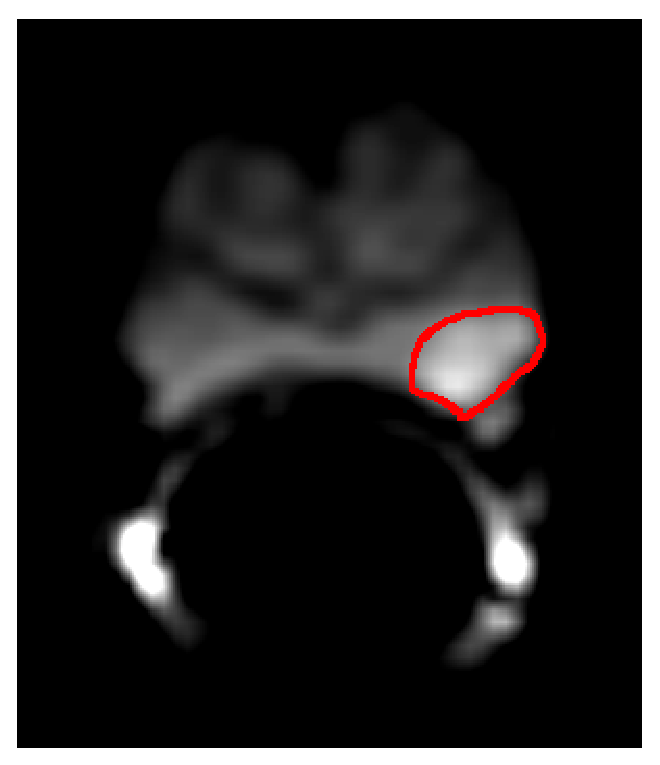
\includegraphics[height=0.2\textheight]{02_background/figures/dwi/dwi_cancer.eps}} \hfill
	\subfigure[\ac{adc} map computer. The cancer corresponds to the low \ac{si} region highlighted in red.]{\label{subfig:adc}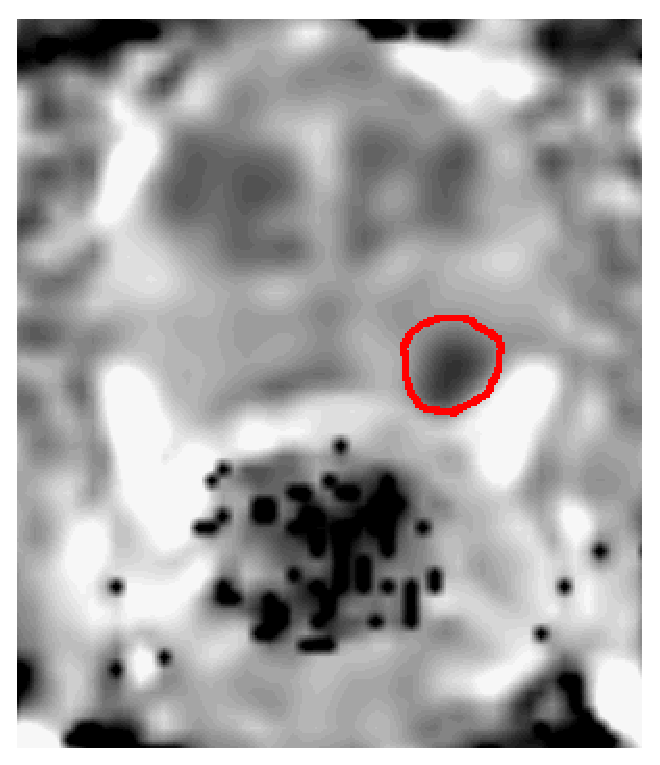
\includegraphics[height=0.2\textheight]{02_background/figures/dwi/adc_cancer.eps}}
	\hspace*{\fill}
	\caption{Illustration of of \ac{dw}-\ac{mri} and \ac{adc} map. The signal intensity corresponding to cancer are inversely correlated on these two types of imaging techniques.}
	\label{fig:dwi}
\end{figure}

%ADC map
\item[$-$] \textbf{\textit{\ac{adc} Map:}} The \ac{nmr} signal measured for \ac{dw} \ac{mri} images is not only affected by diffusion as shown in \acs{eq} \eqref{eq:t2dif}. However, the signal drop (\acs{eq} \eqref{eq:dif}) is formulated such that the only variable is the acquisition parameter $b$ (\cite{LeBihan1986}). The \ac{adc} is considered as a ``pure'' diffusion coefficient and can be extracted to build a quantitative map.

From \acs{eq} \ref{eq:t2dif}, it is clear that performing multiple acquisitions only varying $b$ will not have any effect on the term  $M_{x,y}(0) \exp \left( - \frac{t}{\text{T}_2} \right)$. Thus, \acs{eq} \ref{eq:t2dif} can be rewritten as:

\begin{equation}
	S(b) = S_0 \exp \left( -b \times \text{ADC} \right) \ .
	\label{eq:t2adcrew}
\end{equation}

To compute the \ac{adc} map, a minimum of two acquisitions are necessary: (i) for $b_0=0$ s.mm$^{-2}$ where the measured signal is equal to $S_0$, and (ii) $b_1>0$ s.mm$^{-2}$ (typically $1000$ s.mm$^{-2}$). Then, the \ac{adc} map can be computed as:

\begin{equation}
	\text{ADC} = - \frac{\ln \left( \cfrac{S(b_1)}{S_0} \right) }{b_1} \ .
	\label{eq:adcres1}
\end{equation}

More accurate computation of the \ac{adc} map can be obtained by performing several acquisitions with different values for the parameter $b$ and performing a semi-logarithmic linear fitting using the model presented in \acs{eq} \eqref{eq:t2adcrew}.

Regarding the appearance of the \ac{adc} maps, it was previously stated that by increasing the value of $b$, the signal of \ac{cap} tissue increases significantly. From \acs{eq} \eqref{eq:adcres1}, it can be shown that tissue appearance in the ADC map will be the inverse of \ac{dw} \ac{mri} images. Then, \ac{cap} tissue is associated with low-\ac{si} whereas healthy tissue appears brighter as depicted in Fig.~\ref{subfig:adc} (\cite{Barentsz2012}).

Similar to the gain achieved by \ac{dw} \ac{mri}, diagnosis using \ac{adc} map combined with \ac{t2w} \ac{mri} significantly outperforms \ac{t2w} \ac{mri} alone (\cite{Doo2012,Choi2007}). Moreover, it has been shown that \ac{adc} is correlated with \ac{gs} (\cite{Hambrock2011, Itou2011, Peng2013}).

However, some tissues of the \ac{cg} zone mimic \ac{cap} with low-\ac{si} (\cite{Kirkham2006}) and image distortion can arise due to haemorrhage (\cite{Choi2007}). It has also been noted that a high variability of the \ac{adc} occurs between different patients making it difficult to define a static threshold to distinguish \ac{cap} from non-malignant tumours (\cite{Choi2007}). 

\begin{figure*}
	\centering
	\hspace*{\fill}
	\subfigure[]{\label{subfig:mrsihea}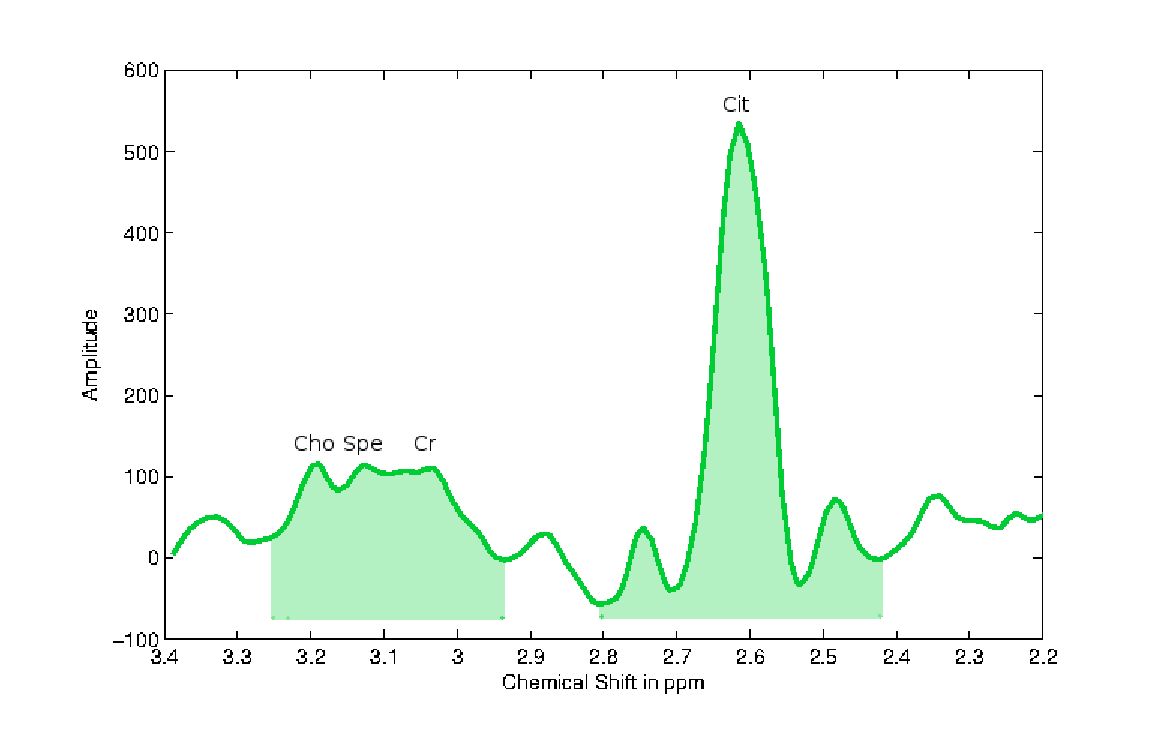
\includegraphics[width=0.45\linewidth]{02_background/figures/mrsi/mrsi_healthy.eps}} \hfill
	\subfigure[]{\label{subfig:mrsican}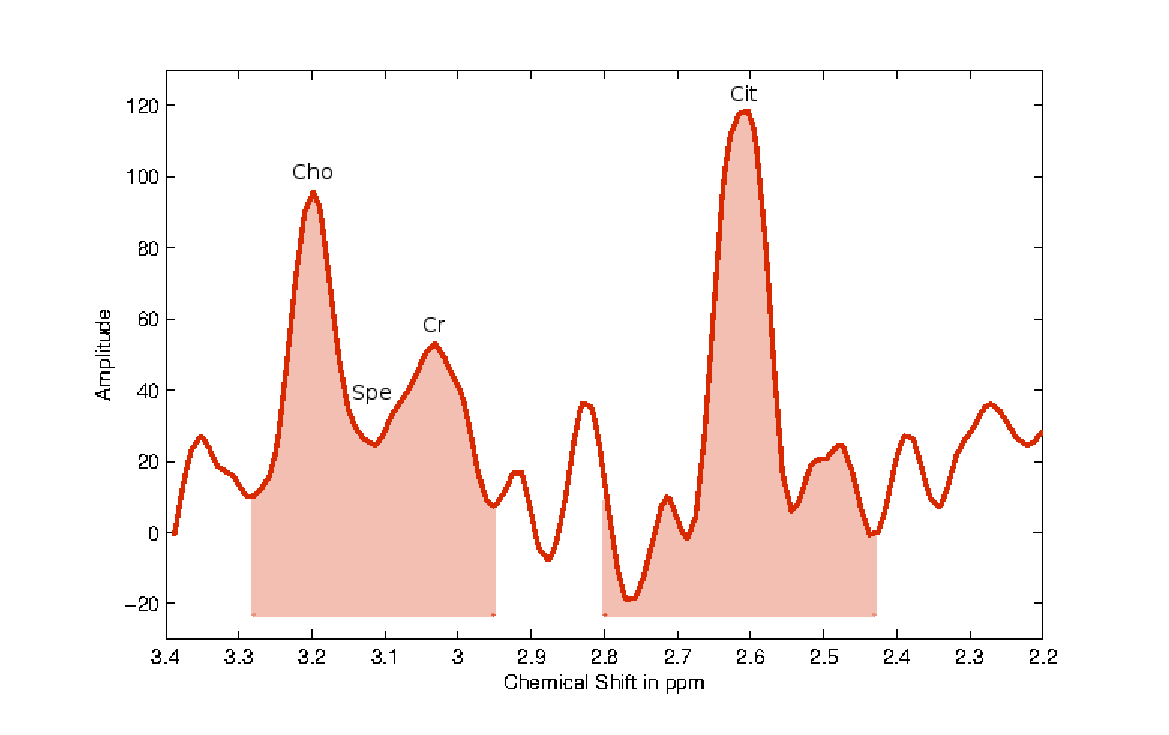
\includegraphics[width=0.45\linewidth]{02_background/figures/mrsi/mrsi_cancer.eps}}
	\hspace*{\fill}
	\caption{Illustration of an \ac{mrsi} spectrum both healthy (Fig. \ref{subfig:mrsihea}) and cancerous (Fig. \ref{subfig:mrsican}) voxel with a 3.0 Tesla \ac{mri}. The highlighted areas corresponds to the related concentration of the metabolites which is computed by integrating the area under each peak. Acronyms: Choline (Cho), Spermine (Spe), Creatine (Cr) and Citrate (Cit).}
	\label{fig:mrsi}
\end{figure*}

%MRSI
\item[$-$] \textbf{\textit{\ac{mrsi}:}} \ac{cap} induces metabolic changes in the prostate compared with healthy tissue. Thus, \ac{cap} detection can be carried out by tracking changes of metabolite concentration in prostate tissue. \ac{mrsi} is an \ac{nmr}-based technique which generates spectra of relative metabolite concentration in \iac{roi}.

In order to track changes of metabolite concentration, it is important to know which metabolites are associated with \ac{cap}. To address this question, clinical studies identified three biological markers: (i) citrate, (ii) choline and (iii) polyamines composed mainly of spermine, and in less abundance of spermidine and putrescine (\cite{Awwad2012,Costello2006,Giskeodegard2013}). 

An increased concentration of choline associated with a decreased concentration of citrate and spermine are related to the presence of \ac{cap} (\cite{Awwad2012,Costello2006,Graaf2000,Giskeodegard2013}).

%Citrate is involved in the production and secretion of the prostatic fluid, and the glandular prostate cells are associated with a high production of citrate enabled by zinc accumulation by these same cells (\cite{Costello2006}). However, the metabolism allowing the accumulation of citrate requires a large amount of energy (\cite{Costello2006}). In contrast, malignant cells do not have high zinc levels leading to lower citrate levels due to citrate oxydation (\cite{Costello2006}). Furthermore, this change results in a more energy-efficient metabolism enabling malignant cells to grow and spread (\cite{Costello2006}).

%An increased concentration of choline is related to \ac{cap} (\cite{Awwad2012}). Malignant cell development requires epigenetic mechanisms resulting in metabolic changes and relies on two mechanisms: DNA methylation and phospholid metabolism which both result in choline uptake, explaining its increased level in \ac{cap} tissue (\cite{Awwad2012}).

%Spermine is also considered as a biological marker in \ac{cap} (\cite{Graaf2000,Giskeodegard2013}). In \ac{cap}, reduction of the ductal volume due to shifts in polyamine homeostasis might lead to a reduced spermine concentration (\cite{Graaf2000}).

To determine the concentration of these biological markers, one has to focus on the \ac{mrsi} modality. % In theory, in presence of a homogeneous magnetic field, identical nuclei precesses at the same operating frequency known as the Lamor frequency (\cite{Haacke1999}). However, \ac{mrsi} is based on the fact that identical nuclei will slightly precess at different frequencies depending on the chemical environment in which they are immersed (\cite{Haacke1999}), a phenomenon known as the \ac{cse} (\cite{Parfait2010}). Given this property, metabolites can be identified and their concentrations can be determined. In this regard, the Fourier transform is used to obtain the frequency spectrum of the \ac{nmr} signal (\cite{Haacke1999,Parfait2010}). 
In each spectrum acquired, each peak is associated with a particular metabolite and the area under each peak corresponds to the relative concentration of this metabolite (see Fig.~\ref{fig:mrsi}) (\cite{Parfait2010}).

Hence, frequencies of interest in regard to \ac{cap} detection and diagnosis should correspond to the earlier mentioned metabolites. Choline and spermine are represented by a single peak at respectively 3.21 ppm and 3.11 ppm (\cite{Verma2010}). Due to the coupling effect, citrate is represented by three or four peaks depending on the magnetic field strength. Citrate ranges from 2.47 ppm to 2.81 ppm with a central frequency at 2.64 ppm (\cite{Verma2010}). Then, relative concentrations of these metabolites are obtained by computing the area under the curve of the spectrum between the lower and upper frequency limits of each peak (see Fig.~\ref{fig:mrsi}). It can be noted that a creatine peak is located at 3.02 ppm and the three metabolite peaks tend to be merged together at clinical magnetic field strengths (see Fig.~\ref{fig:mrsi}) (\cite{Hoeks2011,Graaf2000}).

%Two different quantitative approaches are used to decide or whether not the spectra of \iac{roi} is associated with \ac{cap} classified either as relative quantification or absolute quantification (\cite{Lemaitre2011}).
% In relative quantification, the ratio of choline-polyamines-creatine to citrate is computed. The integral of the signal is computed from choline (cf., 3.21 ppm) to creatine (cf., 3.02 ppm) because the peaks in this region can be merged at clinical magnetic field strengths (see Fig.~\ref{fig:mrsi}) (\cite{Hoeks2011,Graaf2000}). Considering the previous assumption that choline concentration rises and citrate concentration decreases in the presence of \ac{cap}, the ratio computed should be higher in malignant tissue than in healthy tissue. 

%In contrast with relative quantification, absolute quantification measures molar concentrations by normalizing relative concentrations using water as reference (\cite{Lemaitre2011}). In this case, ``true'' concentrations are directly used to differentiate malignant from healthy tissue. However, this method is not commonly used as it requires an additional step of acquiring water signals, inducing time and cost acquisition constraints.

\ac{mrsi} allows examination with high specificity and sensitivity compared to other \ac{mri} modalities (\cite{Choi2007}). Furthermore, it has been shown that combining \ac{mrsi} with \ac{mri} improves detection and diagnosis performance (\cite{Scheidler1999a,Kaji1998,Vilanova2009}). Citrate and spermine concentrations are inversely correlated with the \ac{gs} allowing us to distinguish low from high grade \acp{cap} (\cite{Giskeodegard2013}). However, choline concentration does not provide the same properties (\cite{Giskeodegard2013}).

\newgeometry{margin=.5cm}
\thispagestyle{empty}
\begin{table*}
\centering
\caption{Overview of the different studies reviewed with their main characteristics. Acronyms: number (\#) - image regularization (Img. Reg.).}
\scriptsize
%\begin{adjustwidth}{-2.2cm}{}
\begin{threeparttable}
\renewcommand{\arraystretch}{1}	
	\rowcolors{3}{black!5}{white}	
	\begin{tabular}{|>{\centering\arraybackslash}m{0.7cm}|>{\centering\arraybackslash}m{2.8cm}|>{\centering\arraybackslash}m{0.8cm}|>{\centering\arraybackslash}m{0.8cm}>{\centering\arraybackslash}m{0.8cm}>{\centering\arraybackslash}m{1cm}>{\centering\arraybackslash}m{1cm}|>{\centering\arraybackslash}m{0.7cm}>{\centering\arraybackslash}m{0.7cm}|>{\centering\arraybackslash}m{0.7cm}>{\centering\arraybackslash}m{0.7cm}|>{\centering\arraybackslash}m{0.7cm}>{\centering\arraybackslash}m{0.7cm}>{\centering\arraybackslash}m{0.7cm}|}\hline
	\hiderowcolors
	\multirow{2}{*}{Index} & \multirow{2}{*}{Study} & \# & \multicolumn{4}{c|}{\ac{mri}-modality} & \multicolumn{2}{c|}{Strength of field} & \multicolumn{2}{c|}{Studied zones} & \multicolumn{3}{c|}{\ac{cad} stages} \\ \cline{4-14}
	 & & patients & \ac{t2w} \ac{mri} & \ac{dce} \ac{mri} & \ac{dw} \ac{mri} & \ac{mrsi} & 1.5 T & 3.0 T & \ac{pz} & \ac{cg} & Img. Reg. & \ac{cade} & \ac{cadx} \\ \hline \hline
	 \showrowcolors 
	 	 $[1]$&\cite{Ampeliotis2007} & 25 & \cmark & \cmark & \xmark & \xmark & \cmark & \xmark & \cmark & \xmark & \mmark & \xmark & \cmark \\
	 	 $[2]$&\cite{Ampeliotis2008} & 25 & \cmark & \cmark & \xmark & \xmark & \cmark & \xmark & \cmark & \xmark & \mmark & \xmark & \cmark \\
	 	 $[3]$&\cite{Antic2013} & 53 & \cmark & \xmark & \cmark & \xmark & \cmark & \xmark & \cmark & \cmark & \xmark  & \xmark & \cmark \\
	 	 $[4]$&\cite{Artan2009} & 10 & \cmark & \cmark & \cmark & \xmark & \cmark & \xmark & \cmark & \xmark  & \xmark & \cmark & \cmark \\
	 	 $[5]$&\cite{Artan2010} & 21 & \cmark & \cmark & \cmark & \xmark & \cmark & \xmark & \cmark & \xmark & \mmark & \cmark & \cmark \\
	 	 $[6]$&\cite{Chan2003} & 15 & \cmark & \xmark & \cmark & \xmark & \cmark & \xmark & \cmark & \xmark & \xmark & \xmark & \cmark \\
	 	 $[7]$&\cite{Giannini2013} & 10 & \cmark & \cmark & \cmark & \xmark & \cmark & \xmark & \cmark & \xmark & \cmark & \cmark & \cmark \\
	 	 $[8]$&\cite{Kelm2007} & 24 & \xmark & \xmark & \xmark & \cmark & \cmark & \xmark & \cmark & \cmark & \mmark & \cmark & \cmark \\
	 	 $[9]$&\cite{Langer2009} & 25 & \cmark & \cmark & \cmark & \xmark & \cmark & \xmark & \cmark & \xmark & \mmark & \xmark & \cmark \\
	 	 $[10]$&\cite{Litjens2011} & 188 & \cmark & \cmark & \cmark & \xmark & \xmark & \cmark & \cmark & \xmark & \mmark & \cmark & \cmark \\
	 	 $[11]$&\cite{Litjens2012} & 288 & \cmark & \cmark & \cmark & \xmark & \xmark & \cmark & \cmark & \cmark & \mmark & \cmark & \cmark \\
	 	 $[12]$&\cite{Litjens2014} & 347 & \cmark & \cmark & \cmark & \xmark & \xmark & \cmark & \cmark & \cmark & \mmark & \cmark & \cmark \\
	 	 $[13]$&\cite{Liu2009} & 11 & \cmark & \cmark & \cmark & \xmark & \cmark & \xmark & \cmark & \xmark & \mmark & \cmark & \cmark \\
	 	 $[14]$&\cite{Liu2013} & 54 & \cmark & \cmark & \cmark & \xmark & \xmark & \cmark & \cmark & \cmark & \mmark & \xmark & \cmark \\
	 	 $[15]$&\cite{Lopes2011} & 27 & \cmark & \xmark & \xmark & \xmark & \cmark & \xmark & \cmark & \xmark & \mmark & \cmark & \cmark \\
	 	 $[16]$&\cite{Lv2009} & 55 & \cmark & \xmark & \xmark & \xmark & \cmark & \xmark & \cmark & \xmark & \mmark & \xmark & \cmark \\
	 	 $[17]$&\cite{Matulewicz2013} & 18 & \xmark & \xmark & \xmark & \cmark & \xmark & \cmark & \cmark & \cmark & \xmark & \cmark & \cmark \\ 
	 	 $[18]$&\cite{Mazzetti2011} & 10 & \xmark & \cmark & \xmark & \xmark & \cmark & \xmark & \cmark & \xmark & \mmark & \cmark & \cmark \\
	 	 $[19]$&\cite{Niaf2011} & 23 & \cmark & \cmark & \cmark & \xmark & \cmark & \xmark & \cmark & \xmark & \mmark & \xmark & \cmark \\
	 	 $[20]$&\cite{Niaf2012} & 30 & \cmark & \cmark & \cmark & \xmark & \cmark & \xmark & \cmark & \xmark & \mmark & \xmark & \cmark \\
	 	 $[21]$&\cite{Ozer2009} & 20 & \cmark & \cmark & \cmark & \xmark & \cmark & \xmark & \cmark & \xmark & \mmark & \cmark & \cmark \\
	 	 $[22]$&\cite{Ozer2010} & 20 & \cmark & \cmark & \cmark & \xmark & \cmark & \xmark & \cmark & \xmark & \mmark & \cmark & \cmark \\
	 	 $[23]$&\cite{Parfait2012} & 22 & \xmark & \xmark & \xmark & \cmark & \xmark & \cmark & \cmark & \cmark & \mmark & \cmark & \cmark \\
	 	 $[24]$&\cite{Peng2013} & 48 & \cmark & \cmark & \cmark & \xmark & \xmark & \cmark & \cmark & \cmark & \xmark & \xmark & \cmark \\
	 	 $[25]$&\cite{Puech2009} & 100 & \xmark & \cmark & \xmark & \xmark & \cmark & \xmark & \cmark & \cmark & \xmark & \xmark & \cmark \\
	 	 $[26]$&\cite{Sung2011} & 42 & \xmark & \cmark & \xmark & \xmark & \xmark & \cmark & \cmark & \cmark & \xmark & \cmark & \cmark \\
	 	 $[27]$&\cite{Tiwari2007} & 14 & \xmark & \xmark & \xmark & \cmark & \cmark & \xmark & \cmark & \cmark & \mmark & \cmark & \cmark \\
	 	 $[28]$&\cite{Tiwari2008} & 18 & \xmark & \xmark & \xmark & \cmark & \cmark & \xmark & \cmark & \cmark & \mmark & \cmark & \cmark \\
	 	 $[29]$&\cite{Tiwari2009} & 18 & \xmark & \xmark & \xmark & \cmark & \cmark & \xmark & \cmark & \cmark & \mmark & \cmark & \cmark \\
	 	 $[30]$&\cite{Tiwari2009a} & 15 & \cmark & \xmark & \xmark & \cmark & \cmark & \xmark & \cmark & \cmark & \mmark & \cmark & \cmark \\
	 	 $[31]$&\cite{Tiwari2010} & 19 & \cmark & \xmark & \xmark & \cmark & \cmark & \xmark & \cmark & \cmark & \mmark & \cmark & \cmark \\
	 	 $[32]$&\cite{Tiwari2012} & 36 & \cmark & \xmark & \xmark & \cmark & \cmark & \xmark & \cmark & \cmark & \xmark & \cmark & \cmark \\
	 	 $[33]$&\cite{Tiwari2013} & 29 & \cmark & \xmark & \xmark & \cmark & \cmark & \xmark & \cmark & \cmark & \mmark & \cmark & \cmark \\
	 	 $[34]$&\cite{Viswanath2008} & 16 & \cmark & \xmark & \xmark & \cmark & \cmark & \xmark & \cmark & \cmark & \xmark & \cmark & \cmark \\
	 	 $[35]$&\cite{Viswanath2008a} & 6 & \cmark & \cmark & \xmark & \xmark & \xmark & \cmark & \cmark & \cmark & \mmark & \cmark & \cmark \\
	 	 $[36]$&\cite{Viswanath2009} & 6 & \cmark & \cmark & \xmark & \xmark & \xmark & \cmark & \cmark & \cmark & \cmark & \cmark & \cmark \\
	 	 $[37]$&\cite{Viswanath2011} & 12 & \cmark & \cmark & \cmark & \xmark & \xmark & \cmark & \cmark & \cmark & \mmark & \cmark & \cmark \\
	 	 $[38]$&\cite{Viswanath2012} & 22 & \cmark & \xmark & \xmark & \xmark & \xmark & \cmark & \cmark & \cmark & \cmark & \cmark & \cmark \\
	 	 $[39]$&\cite{Vos2008} & 29 & \cmark & \cmark & \xmark & \xmark & \cmark & \xmark & \cmark & \xmark & \mmark & \xmark & \cmark \\
	 	 $[40]$&\cite{Vos2008a} & 29 & \xmark & \cmark & \xmark & \xmark & \cmark & \xmark & \cmark & \xmark & \mmark & \xmark & \cmark \\
	 	 $[41]$&\cite{Vos2010} & 29 & \cmark & \cmark & \xmark & \xmark & \cmark & \xmark & \cmark & \xmark & \mmark & \xmark & \cmark \\
	 	 $[42]$&\cite{Vos2012} & NA & \cmark & \cmark & \cmark & \xmark & \xmark & \cmark & \cmark & \xmark & \mmark & \cmark & \cmark \\
	 	 \hline
	\end{tabular}
	\begin{tablenotes}
      \footnotesize
      \item Notes:
      \item {\xmark}: not used or not implemented.
      \item {\mmark}: partially implemented.
      \item {\cmark}: used or implemented.
    \end{tablenotes}
\end{threeparttable}
%\end{adjustwidth}
\label{tab:sumpap}
\end{table*}
\restoregeometry


Unfortunately, \ac{mrsi} also presents several drawbacks. First, \ac{mrsi} acquisition is time consuming which prevents this modality from being used in daily clinical practise (\cite{Barentsz2012}). In addition, \ac{mrsi} suffers from low spatial resolution due to the fact that \ac{snr} is linked to the voxel size. However, this issue is addressed by developing new scanners with higher magnetic field strengths such as 7.5 T (\cite{Giskeodegard2013}). Finally, a high variability of the relative concentrations between patients has been observed (\cite{Choi2007}). The same observation was made depending on the zones studied (cf., \ac{pz}, \ac{cg}, base, mid-gland, apex) (\cite{Walker2010,Lemaitre2011}). Due to this variability, it is difficult to use a fixed thresholds in order to differentiate \ac{cap} from healthy tissue.

\end{enumerate}

\subsubsection{Computer-aided systems for \ac{cap}: \ac{cade} - \ac{cadx}} \label{subsubsec:CAD}

As previously mentioned in the introduction (see \acs{sec} \ref{sec:introduction}), \acp{cad} are developed to advise and backup radiologists in their tasks of \ac{cap} detection and diagnosis; \acp{cad} are not aimed to provide fully automatic decisions (\cite{Giger2008}). \acp{cad} can be divided into two different sub-groups either as \ac{cade}, with the purpose to highlight probable lesions in \ac{mri} images, or \ac{cadx}, which focuses on differentiating malignant from non-malignant tumours (\cite{Giger2008}). Moreover, an intuitive approach, motivated by developing a framework combining detection-diagnosis, is to mix both \ac{cade} and \ac{cadx} by using the output of the former mentioned as a input of the latter named. Although the outcomes of these two systems should differ, the framework of both \ac{cad} systems is similar. The \ac{cad} work-flow is presented in \acs{fig} \ref{fig:wkfcad}.

\ac{mri} modalities mentioned in \acs{sec} \ref{subsubsec:mrimrsi} are used as inputs of \ac{cad} for \ac{cap}. % It can be noted that \ac{adc} map is not considered as an input since it is a feature derived from the \ac{dw} \ac{mri} images.
The images acquired from the different modalities show a large variability between patients: the prostate organ can be located at different positions in images (e.g., patient motion, variation of acquisition plan), and the \ac{si} can be corrupted with noise or artefacts during the acquisition process (eg., magnetic field inhomogeneity, use of endorectal coil). To address these issues, the first stage of \ac{cad} is to pre-process multiparametric \ac{mri} images to reduce noise, remove artefacts and standardize the \ac{si}. As most of the later processes will be only focused on the prostate. It is necessary to segment the prostate in each \ac{mri}-modality to define it as \iac{roi}. However, data may suffer from misalignment due to patient motion or different acquisition parameters. Therefore, a registration step is usually performed so that all the previously segmented \ac{mri} images will be in the same reference frame. Registration and segmentation steps can be swapped depending on the strategy chosen.

Some studies do not fully apply the methodology depicted in \acs{fig} \ref{fig:wkfcad}. Details about those can be found in \acs{tab} \ref{tab:sumpap}. Some studies preferred to work directly with raw data in order to demonstrate the robustness of their approaches to noise or artefacts. In some cases, prostate segmentation is performed manually as well as registration. It is also sometimes assumed that no patient motions occur during the acquisition procedure, removing the need of registering the multiparametric \ac{mri} images.

Once the data are regularized, it becomes possible to extract features and classify these data to obtain either the location of possible lesions (\ac{cade}) or/and the malignancy nature of these lesions (\ac{cadx}).

In \iac{cade} framework, \textbf{\textit{possible lesions will be segmented automatically}} and further used as inputs of a \ac{cadx}. Nevertheless, this is not the only case that \ac{cade} frameworks encountered. Some works also used a fused \ac{cade}-\ac{cadx} framework in which a voxel-based delineation approach is used, allowing to obtain the location of the malignant lesions as results. On the other hand, manual lesions segmentation are not considered to be part of \iac{cade}.

\Ac{cadx} is composed of the processes allowing to \textbf{\textit{distinguish malignant from non-malignant tumours}}. In the studies reviewed, \ac{cap} malignancy is defined using the grade of the \ac{gs} determined after post-biopsy or prostatectomy. As presented in Fig. \ref{fig:wkfcad}, \ac{cadx} is usually composed of the three common steps used in classification framework: (i) features detection, (ii) features extraction/selection and (iii) features classification.

As pointed out in the introduction, performance of \ac{cap} detection and diagnosis are affected by observer interpretation and limitations (\cite{Giger2008,Hambrock2013}). \ac{cad} offers a possible solution in order to reduce this variability. As mentioned in the introduction, the effects of \ac{cad} on the observer performance has been studied (\cite{Hambrock2013}), with results showing that \acp{cad} benefit to less-experienced radiologist to perform similarly as experienced radiologist in their tasks (\cite{Hambrock2013}). 

\subsection{Literature classification}

The \ac{cad} review is organized using the methodology presented in \acs{fig} \ref{fig:wkfcad}. Methods embedded in the image regularization framework are presented before to focus on the image classification framework, the later being divided into \ac{cade} and \ac{cadx}. %Pre-processing operations applied to the \ac{mri} data will be classified either as image processing or signal processing. Segmentation will be subdivided into region or model-based methods while registration methods will be classified by reviewing the geometric model, similarity measure and optimizer used.  
\Acl{tab} \ref{tab:sumpap} summarizes the forty-one different \ac{cad} studies reviewed in this paper. The first set of information reported is linked to the data acquisition such as the number of patients included in the study, the modalities acquired as well as the strength of the field of the scanner used. Subsequently, information about the prostate zones considered in the \ac{cad} analysis (\ac{pz} or \ac{cg}) are reported since that detecting \ac{cap} in the \ac{cg} is a more challenging problem and has received particular attention only in recent publications.